\documentclass[UTF8]{ctexart}
\usepackage[a4paper,margin=1in]{geometry}
\usepackage{enumitem}
\setlist[itemize]{leftmargin=2em}
\setlength{\parskip}{0.5em}
\usepackage{graphicx}
\usepackage{float}
\begin{document}
\section{HSTU(Meta)}
\subsection{现有算法存在问题：}  
\begin{itemize}
    \item 传统推荐系统扩展性的瓶颈——即性能提升饱和的问题
    \item 推荐系统中的特征通常缺乏类似自然语言那样的显式结构
    \item 推荐系统面对的是持续变化的十亿级词表
    \item 计算成本是支撑大规模序列模型的主要瓶颈
\end{itemize}

\subsection{算法简介：}
\begin{itemize}
    \item 将召回任务建模成一个序列预测问题，根据用户过去的交互历史，从当前的候选物品池选出预测概率最高的物料。当下一个token是负样本或者不是item，则对应掩码设置为0
    \item 不再将 item 和 action 视为一个整体事件，而是将它们拆分并交错插入到时间序列中，在item位置进行预测，在action位置，Loss进行掩码，不进行预测
    \item 逐点聚合注意力、通过Stochastic Length（SL，主动对厂里是进行稀疏抽样）增加稀疏性、简化Transformer结构
    \item M-FALCON使模型复杂度能够随着候选数线性扩展
\end{itemize}

\begin{figure}[H]
    \centering
    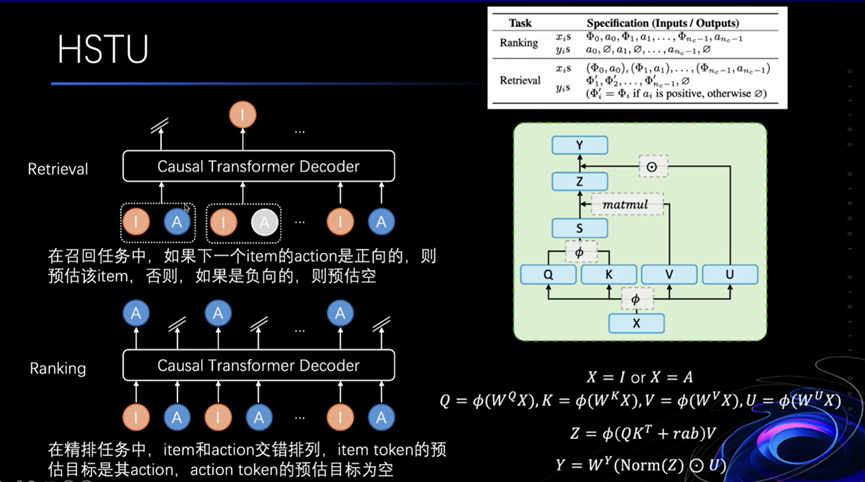
\includegraphics[width=0.85\textwidth, height=0.25\textheight]{1.png} 
    \caption{HSTU算法框架图}
\end{figure}

\subsection{创新点：}
\begin{itemize}
    \item 把推荐重新表述成生成式的序列转导任务，再用 HSTU 作为统一编码器
    \item 将异构的稀疏特征、行为序列与部分数值信息统一到一个可被序列模型处理的结构化时间序列
    \item softmax 更适合静态、相对稳定的词表，而对推荐这种非平稳、持续变化的词表并不理想；pointwise 设计能够更好保留“相关历史出现了多少次”这种强信号，也更适合流式动态词表
    \item 在注意力机制角度，HSTU放弃 Softmax，以保留对推荐至关重要的“强度”信息，同时引入门控 U，以一种极为高效的方式实现了复杂的特征交互
\end{itemize}

\newpage

\section{OneRec（快手）}
\subsection{现有算法存在问题：}  
\begin{itemize}
    \item 将各级排序器视为相互独立的模块，每个独立阶段的效果都会成为后续阶段性能的上界，从而限制了整个排序系统的最终表现
    \item 当前生成模型仍主要扮演召回阶段的选择器角色，因为它们的推荐精度尚不能达到精心设计的多级级联排序系统的水平
    \item RLHF（基于人类反馈的强化学习）存在训练不稳定和效率较低等问题
\end{itemize}

\subsection{算法简介：}
\begin{itemize}
    \item OneRec将用户的正向历史行为序列H作为输入，输出是一个视频列表，即一个会话S。对于输入的每一个视频$v_i$，使用与真实用户-物品行为分布对齐的多模态嵌入$e_i$进行表示。（现有生成式推荐框架通常在预训练多模态表示的基础上，使用 RQ-VAE
将嵌入编码为语义 token。然而，这种方法由于编码分布不平衡，会出现所谓的“沙漏现
象”：RQ 量化后的码字使用非常不均衡，很多 code 几乎没人用，少数 code 被大量样本挤占）本文采用多层均衡量化机制，利用残差 K-means 量化算法对$e_i$进行变换
    \item 会话级生成方法：在解码器中的前馈神经网络FNN替换为MoE架构，在目标会话语义ID上使用交叉熵损失进行next-token prediction
    \item 奖励模型训练：$R(u,S)$表示用户u对会话S的偏好程度，u和vi依次逐点相乘得到目标感知h，再通过自注意力层相互交互，以融合不同物品间的必要信息，使用不同tower对多个目标奖励进行预测
    \item 迭代偏好对齐：先对每个用户u通过beam search（束搜索） 生成 N 个不同响应$S_u^n$，随后利用奖励模型为每一个响应计算奖励，选择奖励值最高和最低的构造偏好数据集。在给定这些偏好对后，我们训练新模型$M_{t+1}$，结合DPO损失目标函数从偏好对中学习。
\end{itemize}

\begin{figure}[H]
    \centering
    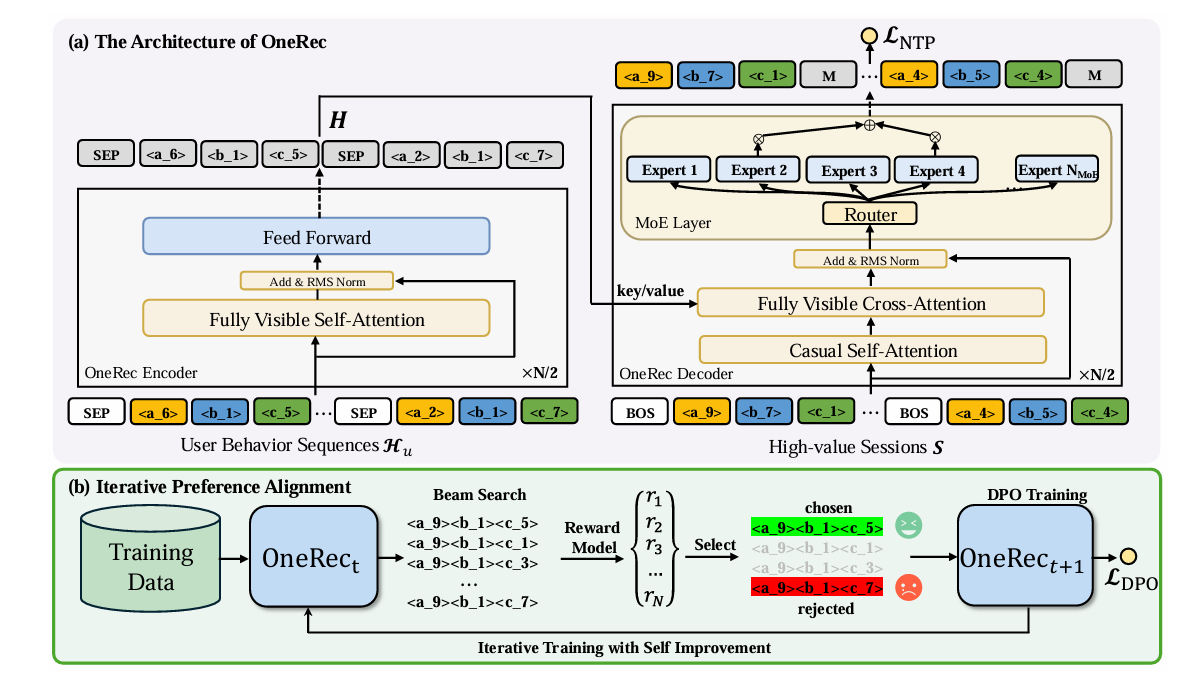
\includegraphics[width=0.75\textwidth, height=0.28\textheight]{2.png} 
    \caption{OneRec算法框架图}
\end{figure}

\subsection{创新点：}
\begin{itemize}
    \item 提出OneRec，一种单阶段生成式推荐框架，这是工业界最早一批能够使用统一生成模型处理物品推荐、并显著超过传统多阶段排序流水线的方案之一。
    \item 通过会话级生成方式强调了模型容量与目标物品上下文信息的重要性，该方式既提高了预测准确性，也增强了生成物品的多样性
    \item 提出一种基于个性化奖励模型的自困难负样本选择策略，并结合直接偏好优化，提高了OneRec 在更广泛用户偏好上的泛化能力
\end{itemize}


\section{OneRec-V2}
\subsection{现有算法存在问题：}  
\begin{itemize}
    \item V1的编码器–解码器架构中的计算分配低效，其中97.66\%的资源消耗在序列上下文编码而非生成阶段，这限制了模型扩展
    \item 仅依赖奖励模型的强化学习存在局限，包括采样效率较低（只能对一小部分用户采样，以近似全局行为），以及由于智能体奖励信号而引发潜在的奖励黑客问题（略模型可能学到的不是“真正让用户更满意的行为”，而是“如何利用奖励模型的偏差、漏洞或伪相关特征，把分数刷高”）
\end{itemize}

\subsection{惰性仅解码器架构简介：}
\begin{itemize}
    \item 上下文处理器：用户画像与行为等异构输入会被拼接成统一序列，即上下文（context=$[C_0,\cdots,C_{S_{kv}\cdot L_{kv}-1}]$）。随后，上下文表示会被变换为供注意力机制使用的分层键值对。我们沿特征维度切分上下文张量，以生成$L_{kv}$ 组键值对$\{(k_0,v_0),\cdots ,{k_{L_{kv}-1},v_{L_{kv}-1}}\}$
    \item Tokenizer：对于每个目标物品，我们采用语义分词器生成3个语义ID，以刻画物品的多方面属性在训练过程中，我们使用前2个ID，并在序列前加上起始符BOS
    \item 块结构：惰性解码器Transformer块包含：交叉注意力、自注意力与前馈网络（在较深层中用MoE模块替换稠密前馈网络）
    \item 惰性交叉注意力：KV共享，多个惰性解码器块共享同一组由上下文处理器产生的键值对，对于第l层，对应索引为：
    $$ l_{kv}=[\frac{l\cdot L_{kv}}{N_{layer}}] $$
    \item 分组查询注意力：查询投影仍保持$H_q=d_{model}/d_{head}$个注意力头，而键值对仅使用$G_{kv}<H_q$个头。
    \item 在训练时，我们最大化目标物品语义ID序列$[s_1,s_2,s_3]$的似然。、
\end{itemize}

\begin{figure}[H]
    \centering
    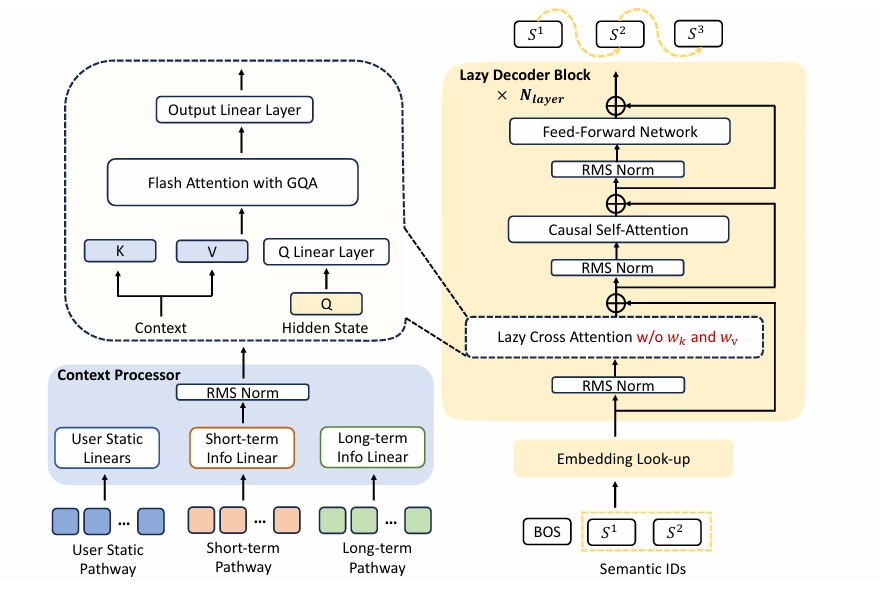
\includegraphics[width=0.85\textwidth, height=0.3\textheight]{3.png} 
    \caption{OneRec-V2算法————惰性仅解码器架构框架图}
\end{figure}

\subsection{基于真实用户交互的偏好对齐简介：}
\begin{itemize}
    \item 时长感知奖励塑形：将目标视频的播放时长，与同一用户历史中“时长相近”的视频进行比较，对播放时长进行归一化。（将视频按时长进行分桶，计算桶内分位数作为得分，25\%分位点以上且没有点踩作为正样本$A_i=+1$，点踩为负样本$A_i=-1$，其余样本被过滤掉$A_i=0$）
    \item 强化学习：提出新的强化学习方法GBPO（Gradient-Bounded Policy Optimization，梯度有界策略优化）——传统强化学习token概率$\pi_\theta$越小，梯度越大（因为Loss要对$\theta$求梯度），正样本情况下这是合理的，但在负样本情况下梯度过大容易崩塌。——GBPO在负样本情况下，当$\pi_\theta$很小时，增大分母；在正样本情况下，当$\pi_\theta$很大时，分母也变大。
\end{itemize}

\begin{figure}[H]
    \centering
    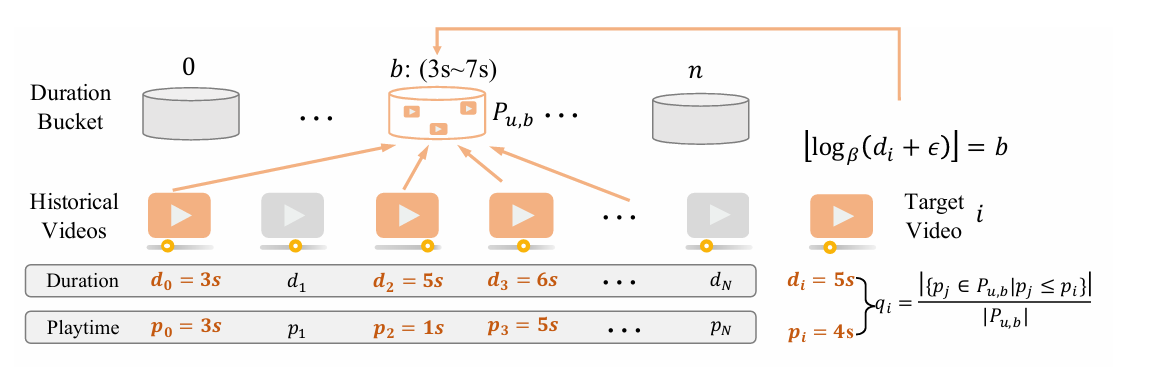
\includegraphics[width=0.85\textwidth, height=0.2\textheight]{4.png} 
    \caption{OneRec-V2算法————时长感知奖励塑形框架图}
\end{figure}

\subsection{创新点：}
\begin{itemize}
    \item 惰性仅解码器架构（Lazy Decoder-Only Architecture）：该架构采用精简的仅解码器设计，消除了编码器瓶颈并简化了交叉注意力，使总计算量降低94\%、训练资源降低90\%。这种效率使模型能够成功扩展到8B参数规模；更重要的是，其
收敛损失与经验扩展律高度吻合
    \item 基于真实用户交互的偏好对齐（Preference Alignment with Real-World UserInteractions）——该框架以用户反馈为驱动
    \item 时长感知奖励塑形：通过考虑视频时长差异，缓解原始观看时长信号中的固有偏差，使奖励更准确地反映内容质量而非时长本身
    \item 自适应比率裁剪：在保证策略优化收敛性的同时有效降低训练方差，样本完全利用——保留所有样本的梯度，鼓励模型进行更丰富的探索；有界梯度稳定化——用BCE（二元交叉熵）损失中更稳定的梯度为强化学习梯度设界，从
而增强训练稳定性。
\end{itemize}


\section{MTGR（美团）}
\subsection{现有算法存在问题：}  
\begin{itemize}
    \item 生成式推荐放弃传统模型中精心构造的交叉特征（候选项与用户之间），这种做法会显著损害模型性能
    \item 扩展用户模块，不能增强用户与物品之间的特征交互
    \item 扩展交叉模块，计算开销会随着候选项数量线性增长，系统时延不可接受
\end{itemize}

\subsection{算法简介：}
\begin{itemize}
	\item 传统第i个用户-候选项样本可表示为$D_i=[U,S,R,C_i,I_i]$，其中U表示用户画像特征，Ui都是标量；S是历史交互序列，Si是一个embedding向量；R是最近交互；C是交叉特征；I是候选项特征，在不同用户之间共享
    \item 对于候选样本中第i个样本，将特征组织为$D_i=[U,S,R,[C_i,I_i]]$，具体而言，把交叉特征C看作候选项特征的一部分，聚合后的样本共享一份用户表示$(U,S,R)$，形式化的，同一用户的特征表示为：
    $$ D=[U,S,R,[C,I]_1,\cdots,[C,I]_k] $$
    全部转换为统一维度的token，连接形成一个长token序列$Feat_D \in R^{(N_U+N_S+N_R+N_I)\times d_{model}}$
    \item 统一HSTU编码器：输入序列X按照不同域进行“组层归一化”，然后对归一化后的输入进行4组不同投影得到KQVU，Value计算如下：
    $$ V'=\frac{silu(K^TQ)}{(N_U+N_S+N_R+N_I)}MV  $$
    其中M为定制掩码，随后用U和V‘点乘，再次组层归一化，加入残差模块后接上一个MLP：
    $$ X=MLP(GroupLN(V'\odot U))+X $$
    \item 动态掩码使用因果掩码进行序列建模效果无提升且会造成信息泄露。静态信息（U，S）来自聚合窗口之前，不会引发因果性错误，而R是动态的，会实时纳入用户交互信息。因此，MTGR对静态序列使用全注意力，对R使用带动态掩码的自回归注意力（每个token只对其之后出现的token 可见，这其中也包括候选项token），而对候选项之间使用对角掩码。
    \item 动态哈希表：采用解耦哈希表架构，将Key存储与Value存储分离。
    \item 负载均衡（拼接短序列）：常规做法是序列打包技术，将多个短序列拼接为更长序列。然而，这种方法要求仔细调整掩码，实现代价较高。算法引入动态BS，根据输入数据的实际序列长度动态调整每张GPU的本地BS，从而使各GPU的计算负载保持相近。调整了梯度聚合策略，使每张GPU的梯度按照其BS加权，从而保证与固定BS情形下的计算逻辑一致
\end{itemize}

\begin{figure}[H]
    \centering
    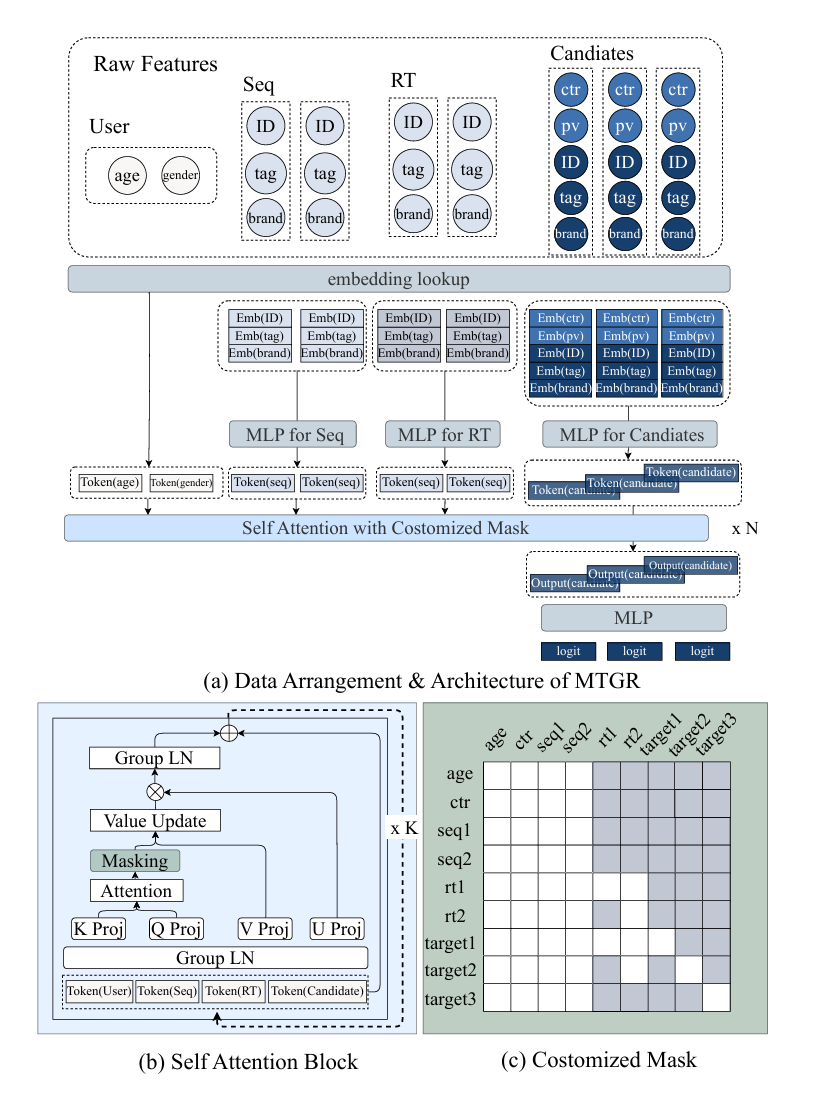
\includegraphics[width=0.75\textwidth, height=0.45\textheight]{5.png} 
    \caption{MTGR算法框架图}
\end{figure}

\subsection{创新点：}
\begin{itemize}
    \item 保留原始深度学习推荐模型（DLRM）的特征，包括交叉特征
    \item 通过用户级压缩实现训练与推理加速，从而保证高效扩展
    \item 组层归一化（Group-Layer Normalization,GLN），以增强不同语义空间中的编码效果
    \item 提出动态掩码策略以避免信息泄漏
\end{itemize}






\end{document}